\documentclass[tikz,border=4pt]{standalone}
\usepackage[T1]{fontenc}
\usepackage{lmodern}
\renewcommand{\familydefault}{\sfdefault}
\usetikzlibrary{shapes.geometric,positioning,arrows.meta,calc,fit,backgrounds,decorations.pathreplacing}
\tikzset{
  node distance=6mm,
  every node/.style={font=\footnotesize,align=center,execute at begin node={\hyphenpenalty=10000\relax}},
  base/.style={draw=gray!60,fill=gray!12,minimum height=7mm,inner sep=2pt},
  term/.style={base,rounded corners=3.5mm,text width=30mm},
  proc/.style={base,text width=32mm},
  err/.style={base,text width=30mm,fill=gray!22},
  io/.style={base,trapezium,trapezium left angle=72,trapezium right angle=108,trapezium stretches=true,text width=28mm},
  dec/.style={base,diamond,aspect=2.4,text width=27mm,inner sep=0pt},
  % predefined process: a call to another procedure
  sub/.style={proc,inner xsep=3mm,path picture={
    \draw[gray!60] ([xshift=1.5mm]path picture bounding box.north west)--([xshift=1.5mm]path picture bounding box.south west)
                   ([xshift=-1.5mm]path picture bounding box.north east)--([xshift=-1.5mm]path picture bounding box.south east);}},
  go/.style={-{Stealth[length=2mm]},draw=gray!55!black},
  lab/.style={font=\scriptsize,fill=white,inner sep=1pt},
  frame/.style={draw=gray!60,dashed,rounded corners=2mm,inner sep=3mm},
  % memory diagrams
  cell/.style={draw=gray!60,fill=gray!12,minimum height=7mm,inner sep=1pt,font=\scriptsize},
  hot/.style={cell,fill=gray!35},
  note/.style={font=\scriptsize,text=gray!30!black},
}

\begin{document}
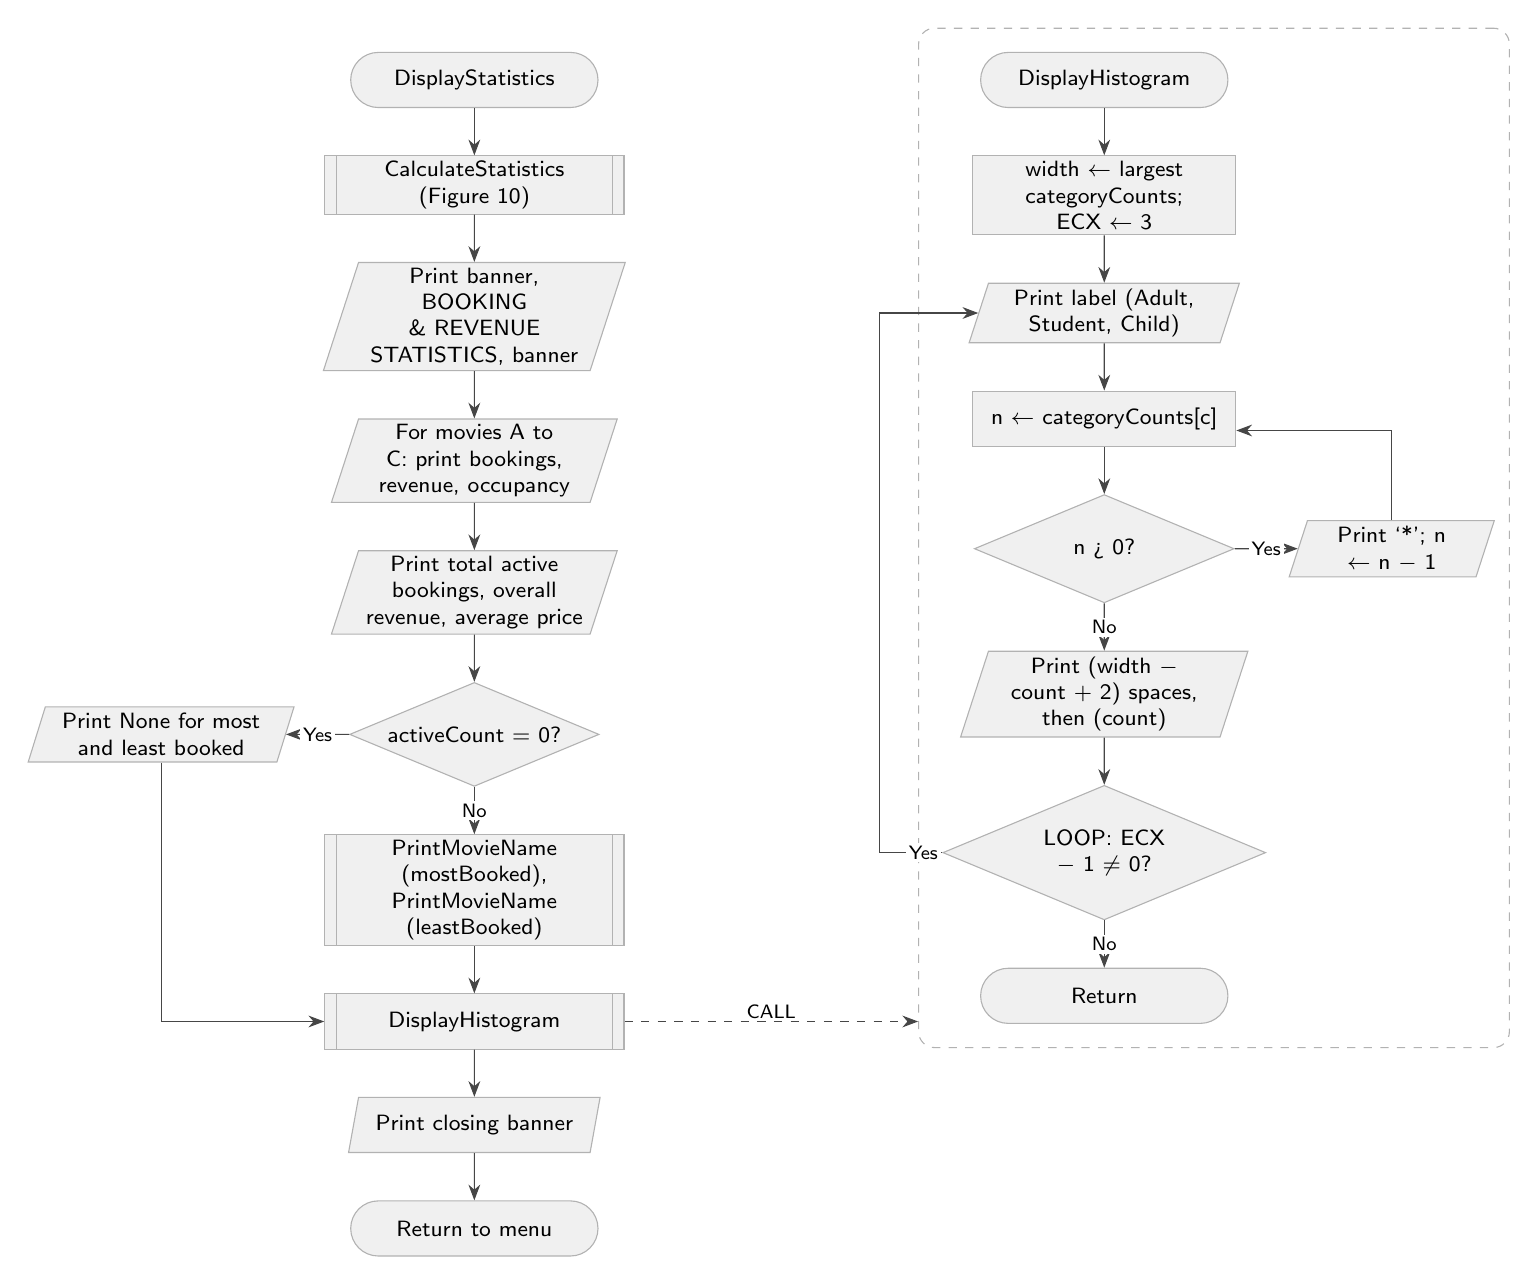
\begin{tikzpicture}
\node[term] (s) {DisplayStatistics};
\node[sub,below=of s] (c) {CalculateStatistics (Figure 10)};
\node[io,below=of c] (b) {Print banner, BOOKING \& REVENUE STATISTICS, banner};
\node[io,below=of b] (m) {For movies A to C: print bookings, revenue, occupancy};
\node[io,below=of m] (t) {Print total active bookings, overall revenue, average price};
\node[dec,below=of t] (d) {activeCount = 0?};
\node[io,left=8mm of d] (no) {Print None for most and least booked};
\node[sub,below=of d] (mv) {PrintMovieName (mostBooked), PrintMovieName (leastBooked)};
\node[sub,below=of mv] (h) {DisplayHistogram};
\node[io,below=of h] (bb) {Print closing banner};
\node[term,below=of bb] (e) {Return to menu};
\draw[go] (s)--(c);
\draw[go] (c)--(b);
\draw[go] (b)--(m);
\draw[go] (m)--(t);
\draw[go] (t)--(d);
\draw[go] (d)--node[lab]{Yes}(no);
\draw[go] (no)|-(h.west);
\draw[go] (d)--node[lab]{No}(mv);
\draw[go] (mv)--(h);
\draw[go] (h)--(bb);
\draw[go] (bb)--(e);
% DisplayHistogram
\node[term] (hs) at ($(s)+(80mm,0)$) {DisplayHistogram};
\node[proc,below=of hs] (w) {width $\leftarrow$ largest categoryCounts; ECX $\leftarrow$ 3};
\node[io,below=of w] (lb) {Print label (Adult, Student, Child)};
\node[proc,below=of lb] (n) {n $\leftarrow$ categoryCounts[c]};
\node[dec,below=of n] (dn) {n > 0?};
\node[io,right=8mm of dn,text width=20mm] (st) {Print `*'; n $\leftarrow$ n $-$ 1};
\node[io,below=of dn] (pd) {Print (width $-$ count + 2) spaces, then (count)};
\node[dec,below=of pd] (lp) {LOOP: ECX $-$ 1 $\neq$ 0?};
\node[term,below=of lp] (he) {Return};
\draw[go] (hs)--(w);
\draw[go] (w)--(lb);
\draw[go] (lb)--(n);
\draw[go] (n)--(dn);
\draw[go] (dn)--node[lab]{Yes}(st);
\draw[go] (st.north)|-([yshift=-1.5mm]n.east);
\draw[go] (dn)--node[lab]{No}(pd);
\draw[go] (pd)--(lp);
\draw[go] (lp.west)--node[lab,pos=.3]{Yes}++(-8mm,0)|-(lb.west);
\draw[go] (lp)--node[lab]{No}(he);
\begin{scope}[on background layer]
\node[frame,fit=(hs)(w)(lb)(n)(dn)(st)(pd)(lp)(he)] (box) {};
\end{scope}
\draw[go,dashed] (h.east)--node[lab,above]{CALL}(h.east -| box.west);
\end{tikzpicture}
\end{document}
